\documentclass{beamer}

\usepackage[utf8]{inputenc}
\usepackage{default}
\usepackage[OT4]{polski}
\usepackage[normalem]{ulem}
\usepackage{color}
\usepackage{graphicx}
\usepackage{listings}
\usepackage{fancyvrb}
\usepackage{tikz}
\usepackage{listings}
\usepackage{hyperref}
\usetheme{Warsaw}

\graphicspath{ {files/} }

\tikzstyle{line} = [draw, -latex]
\tikzstyle{path} = [draw, -latex, style={decorate,decoration={snake}}]
\tikzstyle{state} = [circle,draw=black,minimum size=0.6cm]
\tikzstyle{finish_state} = [circle,draw=black,double=white,double distance=1pt,minimum size=0.9cm]
\usetikzlibrary{shapes,arrows,automata,decorations.pathmorphing}

\definecolor{dkgreen}{rgb}{0,0.6,0}
\definecolor{gray}{rgb}{0.5,0.5,0.5}
\definecolor{mauve}{rgb}{0.58,0,0.82}

\lstset{
  language=C,
  aboveskip=3mm,
  belowskip=3mm,
  showstringspaces=false,
  columns=flexible,
  basicstyle={\small\ttfamily},
  numbers=none,
  numberstyle=\tiny\color{gray},
  keywordstyle=\color{blue},
  commentstyle=\color{dkgreen},
  stringstyle=\color{mauve},
  breaklines=true,
  breakatwhitespace=true,
  tabsize=4,
  escapeinside=``
}

\lstdefinelanguage
	[x86fp]{Assembler}
	[x86masm]{Assembler} 
	{morekeywords={movss}}
   
\lstdefinelanguage
   [my]{C}
   []{C} 
   {morekeywords={bool}}
   
   
   \lstdefinelanguage{llvm}{
  morecomment = [l]{;},
  morestring=[b]", 
  sensitive = true,
  classoffset=0,
  morekeywords={
    define, declare, global, constant,
    internal, external, private,
    linkonce, linkonce_odr, weak, weak_odr, appending,
    common, extern_weak,
    thread_local, dllimport, dllexport,
    hidden, protected, default,
    except, deplibs,
    volatile, fastcc, coldcc, cc, ccc,
    x86_stdcallcc, x86_fastcallcc,
    ptx_kernel, ptx_device,
    signext, zeroext, inreg, sret, nounwind, noreturn,
    nocapture, byval, nest, readnone, readonly, noalias, uwtable,
    inlinehint, noinline, alwaysinline, optsize, ssp, sspreq,
    noredzone, noimplicitfloat, naked, alignstack,
    module, asm, align, tail, to,
    addrspace, section, alias, sideeffect, c, gc,
    target, datalayout, triple,
    blockaddress
  },
  classoffset=1, keywordstyle=\color{purple},
  morekeywords={
    fadd, sub, fsub, mul, fmul,
    sdiv, udiv, fdiv, srem, urem, frem,
    and, or, xor,
    icmp, fcmp,
    eq, ne, ugt, uge, ult, ule, sgt, sge, slt, sle,
    oeq, ogt, oge, olt, ole, one, ord, ueq, ugt, uge,
    ult, ule, une, uno,
    nuw, nsw, exact, inbounds,
    phi, call, select, shl, lshr, ashr, va_arg,
    trunc, zext, sext,
    fptrunc, fpext, fptoui, fptosi, uitofp, sitofp,
    ptrtoint, inttoptr, bitcast,
    ret, br, indirectbr, switch, invoke, unwind, unreachable,
    malloc, alloca, free, load, store, getelementptr,
    extractelement, insertelement, shufflevector,
    extractvalue, insertvalue,
  },
  alsoletter={\%},
  keywordsprefix={\%},
}

\begin{document}
	\begin{frame}
		\frametitle{ZPP -- NianioLang}
		Prezentacja -- kompilatory
		
		22.03.2018
	\end{frame}
	
	\begin{frame}
		\frametitle{Kompilator}
		Program, który czyta kod napisany w jednym języku (\textit{źródłowym})
		i tłumaczy go na równoważny kod w drugim języku (\textit{wynikowym})
	\end{frame}
	
	\begin{frame}
		\frametitle{Etapy kompilacji}
		\begin{itemize}
			\item Analiza leksykalna
			\item Analiza składniowa
			\item Analiza semantyczna
			\item \textit{Generacja kodu pośredniego}
			\item \textit{Optymalizacja}
			\item Generacja kodu
		\end{itemize}
	\end{frame}
	
	\begin{frame}[fragile]
		\frametitle{Analiza leksykalna}
		\begin{columns}
			\begin{column}{0.5\textwidth}
				\center{Kod źródłowy}\newline\newline
			\end{column}
			\begin{column}{0.5\textwidth}
				\center{Tokeny}\newline\newline
			\end{column}
		\end{columns}
		\begin{columns}
			\begin{column}{0.45\textwidth}
				\begin{lstlisting}
// Ustaw wartosc a
var a = 4 + 0.2
				\end{lstlisting}
			\end{column}
			\begin{column}{0.1\textwidth}
$\Rightarrow$
			\end{column}
			\begin{column}{0.45\textwidth}
				\textbf{keyword}(\texttt{var}),\newline
				\textbf{id}(\texttt{a}),\newline
				\textbf{operator}(\texttt{=}),\newline
				\textbf{integer}(\texttt{4}),\newline
				\textbf{operator}(\texttt{+}),\newline
				\textbf{real}(\texttt{0.2})
			\end{column}
		\end{columns}
	\end{frame}
	
	\begin{frame}[fragile]
		\frametitle{Analiza składniowa}
		\begin{columns}
			\begin{column}{0.5\textwidth}
				\center{Tokeny}\newline\newline
			\end{column}
			\begin{column}{0.5\textwidth}
				\center{AST}\newline\newline
			\end{column}
		\end{columns}
		\begin{columns}
			\begin{column}{0.3\textwidth}
				\textbf{keyword}(\texttt{var}),\newline
				\textbf{id}(\texttt{a}),\newline
				\textbf{operator}(\texttt{=}),\newline
				\textbf{integer}(\texttt{4}),\newline
				\textbf{operator}(\texttt{+}),\newline
				\textbf{real}(\texttt{0.2})
			\end{column}
			\begin{column}{0.1\textwidth}
$\Rightarrow$
			\end{column}
			\begin{column}{0.6\textwidth}
				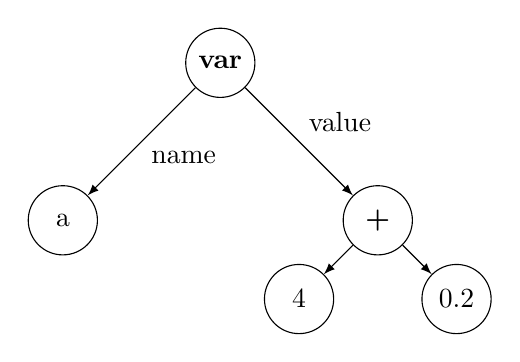
\begin{tikzpicture}
					[scale=1,auto=left]
					\node [state] (var) at (9,10) {\textbf{var}};
					\node [state] (name) at (7,8) {a};
					\node [state] (value) at (11,8) {\textbf{+}};
					\node [state] (left) at (10,7) {4};
					\node [state] (right) at (12,7) {0.2};
					\path [line] (var) to[left] node[auto] {name} (name);
					\path [line] (var) to[left] node[auto] {value} (value);
					\path [line] (value) to[left] node[auto] {} (left);
					\path [line] (value) to[left] node[auto] {} (right);
				\end{tikzpicture}
			\end{column}
		\end{columns}
	\end{frame}
	
	\begin{frame}[fragile]
		\frametitle{Analiza semantyczna}
		\begin{columns}
			\begin{column}{0.5\textwidth}
				\center{AST}\newline\newline
			\end{column}
			\begin{column}{0.5\textwidth}
				\center{AST'}\newline\newline
			\end{column}
		\end{columns}
		\begin{columns}
			\begin{column}{0.45\textwidth}
				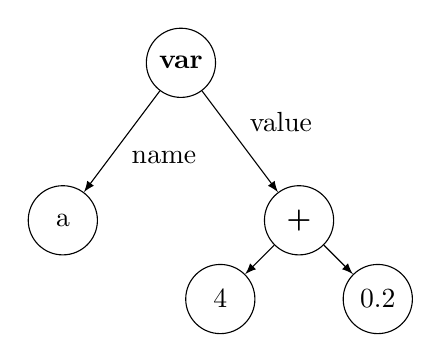
\begin{tikzpicture}
					[scale=1,auto=left]
					\node [state] (var) at (8.5,10) {\textbf{var}};
					\node [state] (name) at (7,8) {a};
					\node [state] (value) at (10,8) {\textbf{+}};
					\node [state] (left) at (9,7) {4};
					\node [state] (right) at (11,7) {0.2};
					\path [line] (var) to[left] node[auto] {name} (name);
					\path [line] (var) to[left] node[auto] {value} (value);
					\path [line] (value) to[left] node[auto] {} (left);
					\path [line] (value) to[left] node[auto] {} (right);
				\end{tikzpicture}
			\end{column}
			\begin{column}{0.1\textwidth}
$\Rightarrow$
			\end{column}
			\begin{column}{0.45\textwidth}
				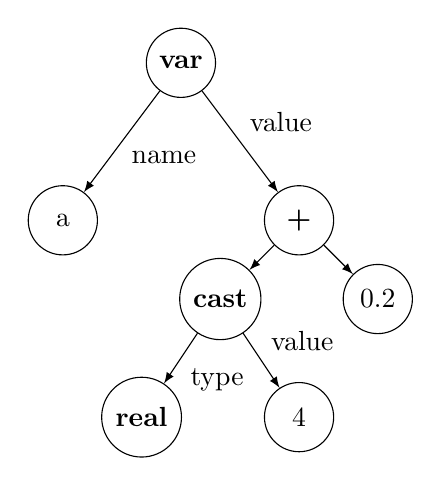
\begin{tikzpicture}
					[scale=1,auto=left]
					\node [state] (var) at (8.5,10) {\textbf{var}};
					\node [state] (name) at (7,8) {a};
					\node [state] (value) at (10,8) {\textbf{+}};
					\node [state] (left_cast) at (9,7) {\textbf{cast}};
					\node [state] (left_value) at (10,5.5) {4};
					\node [state] (left_type) at (8,5.5) {\textbf{real}};
					\node [state] (right) at (11,7) {0.2};
					\path [line] (var) to[left] node[auto] {name} (name);
					\path [line] (var) to[left] node[auto] {value} (value);
					\path [line] (value) to[left] node[auto] {} (left_cast);
					\path [line] (left_cast) to[left] node[auto] {type} (left_type);
					\path [line] (left_cast) to[left] node[auto] {value} (left_value);
					\path [line] (value) to[left] node[auto] {} (right);
				\end{tikzpicture}
			\end{column}
		\end{columns}
	\end{frame}
	
	\begin{frame}[fragile]
		\frametitle{Generacja kodu}
		\begin{columns}
			\begin{column}{0.5\textwidth}
				\center{AST'}\newline\newline
			\end{column}
			\begin{column}{0.5\textwidth}
				\center{Kod wynikowy}\newline\newline
			\end{column}
		\end{columns}
		\begin{columns}
			\begin{column}{0.45\textwidth}
				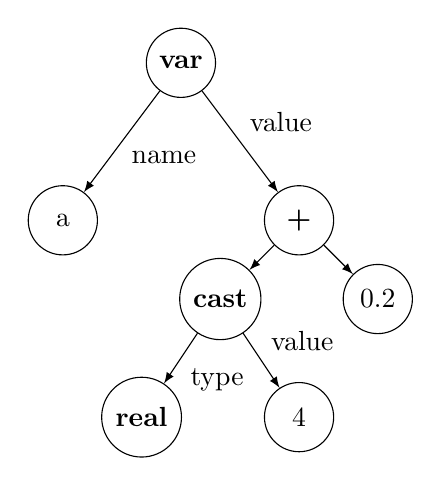
\begin{tikzpicture}
					[scale=1,auto=left]
					\node [state] (var) at (8.5,10) {\textbf{var}};
					\node [state] (name) at (7,8) {a};
					\node [state] (value) at (10,8) {\textbf{+}};
					\node [state] (left_cast) at (9,7) {\textbf{cast}};
					\node [state] (left_value) at (10,5.5) {4};
					\node [state] (left_type) at (8,5.5) {\textbf{real}};
					\node [state] (right) at (11,7) {0.2};
					\path [line] (var) to[left] node[auto] {name} (name);
					\path [line] (var) to[left] node[auto] {value} (value);
					\path [line] (value) to[left] node[auto] {} (left_cast);
					\path [line] (left_cast) to[left] node[auto] {type} (left_type);
					\path [line] (left_cast) to[left] node[auto] {value} (left_value);
					\path [line] (value) to[left] node[auto] {} (right);
				\end{tikzpicture}
			\end{column}
			\begin{column}{0.15\textwidth}
$\Rightarrow\ldots\Rightarrow$
			\end{column}
			\begin{column}{0.40\textwidth}
				\lstset{language=[x86fp]Assembler}
				\begin{lstlisting}
.LC0:
  .long 1082549862
_start:
  movss xmm0, .LC0[rip]
  movss -4[rbp], xmm0
  mov eax, 0
  ret
				\end{lstlisting}
			\end{column}
		\end{columns}
	\end{frame}
	
	\begin{frame}
		\frametitle{Notacja infksowa $\rightarrow$ Notacja postfiksowa}
		\begin{itemize}
			\item Notacja infiksowa: $\texttt{e}_1\ +\ \texttt{e}_2$
			\item Notacja postfiksowa (odwrotna notacja polska): $\texttt{e}_1\ \texttt{e}_2\ +$
			\begin{itemize}
				\item Przykłady:
				\begin{itemize}
					\item \texttt{1 + 2 * 3}\hspace{1em} $\Rightarrow$ \hspace{1em}\texttt{1 2 3 * +}
					\item \texttt{(1 + 2) * 3}\hspace{1em} $\Rightarrow$ \hspace{1em}\texttt{1 2 + 3 * }
				\end{itemize}
				\item Nie wymaga nawiasów
				\item Łatwo obliczać wartość wyrażenia (implementacja na stosie)
				\item Niestety nieczytelna dla ludzi :( 
			\end{itemize}
		\end{itemize}
	\textbf{Napiszmy kompilator!}\newline
	\end{frame}
	
	\begin{frame}
		\frametitle{Definicja składni v1 (Składnia abstrakcyjna)}
			\texttt{wyrażenie $\rightarrow$ wyrażenie + wyrażenie |\newline
			\phantom{wyrażenie $\rightarrow$ }wyrażenie * wyrażenie |\newline
			\phantom{wyrażenie $\rightarrow$ }(wyrażenie) | liczba
		}
		\pause
		\center{\textbf{Jaki jest problem?}}
		\pause
		\center{\texttt{1 + 2 * 3}}
		\vspace{1em}
		\begin{columns}
			\begin{column}{0.5\textwidth}
				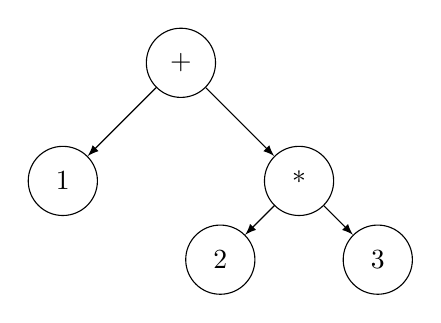
\begin{tikzpicture}
					[scale=1,auto=left]
					\node [state] (+) at (8.5,9.5) {+};
					\node [state] (1) at (7,8) {1};
					\node [state] (*) at (10,8) {*};
					\node [state] (2) at (9,7) {2};
					\node [state] (3) at (11,7) {3};
					\path [line] (+) to[left] node[auto] {} (1);
					\path [line] (+) to[left] node[auto] {} (*);
					\path [line] (*) to[left] node[auto] {} (2);
					\path [line] (*) to[left] node[auto] {} (3);
				\end{tikzpicture}
			\end{column}
			\begin{column}{0.5\textwidth}
				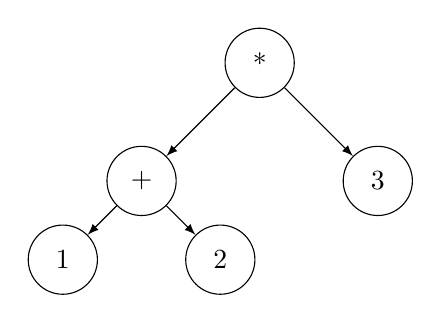
\begin{tikzpicture}
					\node [state] (*) at (8.5,9.5) {*};
					\node [state] (+) at (7,8) {+};
					\node [state] (1) at (6,7) {1};
					\node [state] (2) at (8,7) {2};
					\node [state] (3) at (10,8) {3};
					\path [line] (*) to[left] node[auto] {} (+);
					\path [line] (*) to[left] node[auto] {} (3);
					\path [line] (+) to[left] node[auto] {} (1);
					\path [line] (+) to[left] node[auto] {} (2);
				\end{tikzpicture}
			\end{column}
		\end{columns}
	\end{frame}
	
	\begin{frame}
		\frametitle{Definicja składni v2 (Składnia konkretna)}
		\texttt{wyrażenie $\rightarrow$ skladnik | skladnik + wyrazenie}\newline
		\texttt{składnik $\rightarrow$ czynnik | czynnik * skladnik} \newline
		\texttt{czynnik $\rightarrow$ (wyrażenie) | liczba}
		\pause
		\center{\texttt{1 + 2 * 3}}
		\begin{columns}
			\begin{column}{0.5\textwidth}
				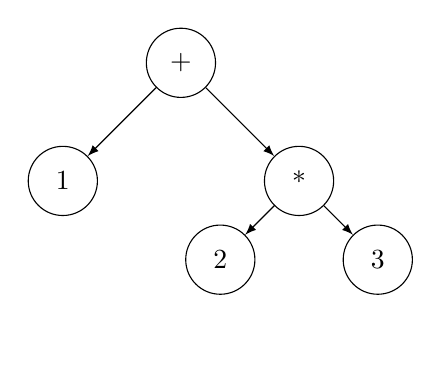
\begin{tikzpicture}
					[scale=1,auto=left]
					\node [state] (+) at (8.5,9.5) {+};
					\node [state] (1) at (7,8) {1};
					\node [state] (*) at (10,8) {*};
					\node [state] (2) at (9,7) {2};
					\node [state] (3) at (11,7) {3};
					\phantom{\draw[red] (10, 7.2) circle (10ex);}
					\path [line] (+) to[left] node[auto] {} (1);
					\path [line] (+) to[left] node[auto] {} (*);
					\path [line] (*) to[left] node[auto] {} (2);
					\path [line] (*) to[left] node[auto] {} (3);
				\end{tikzpicture}
			\end{column}
			\begin{column}{0.5\textwidth}
				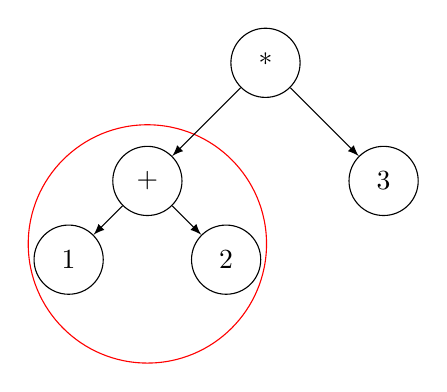
\begin{tikzpicture}
					\node [state] (*) at (8.5,9.5) {*};
					\node [state] (+) at (7,8) {+};
					\node [state] (1) at (6,7) {1};
					\node [state] (2) at (8,7) {2};
					\node [state] (3) at (10,8) {3};
					\draw[red] (7, 7.2) circle (10ex);
					\path [line] (*) to[left] node[auto] {} (+);
					\path [line] (*) to[left] node[auto] {} (3);
					\path [line] (+) to[left] node[auto] {} (1);
					\path [line] (+) to[left] node[auto] {} (2);
				\end{tikzpicture}
			\end{column}
		\end{columns}
	\end{frame}
	
	\begin{frame}
		\frametitle{Definicja składni v2 (Składnia konkretna)}
		\texttt{wyrażenie $\rightarrow$ skladnik | skladnik + wyrazenie}\newline
		\texttt{składnik $\rightarrow$ czynnik | czynnik * skladnik} \newline
		\texttt{czynnik $\rightarrow$ (wyrażenie) | liczba}
		\begin{columns}
			\begin{column}{0.5\textwidth}
				\center{\texttt{1 + 2 * 3}}\newline
			\end{column}
			\begin{column}{0.5\textwidth}
				\center{\texttt{\hspace{2em}(1 + 2) * 3}}\newline
			\end{column}
		\end{columns}
		\begin{columns}
			\begin{column}{0.5\textwidth}
				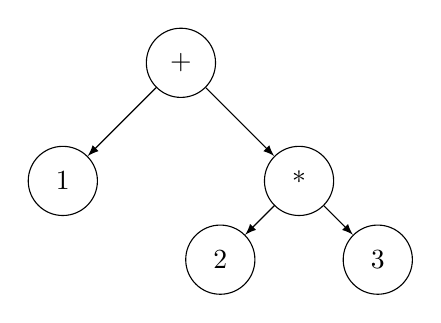
\begin{tikzpicture}
					[scale=1,auto=left]
					\node [state] (+) at (8.5,9.5) {+};
					\node [state] (1) at (7,8) {1};
					\node [state] (*) at (10,8) {*};
					\node [state] (2) at (9,7) {2};
					\node [state] (3) at (11,7) {3};
					\path [line] (+) to[left] node[auto] {} (1);
					\path [line] (+) to[left] node[auto] {} (*);
					\path [line] (*) to[left] node[auto] {} (2);
					\path [line] (*) to[left] node[auto] {} (3);
				\end{tikzpicture}
			\end{column}
			\begin{column}{0.5\textwidth}
				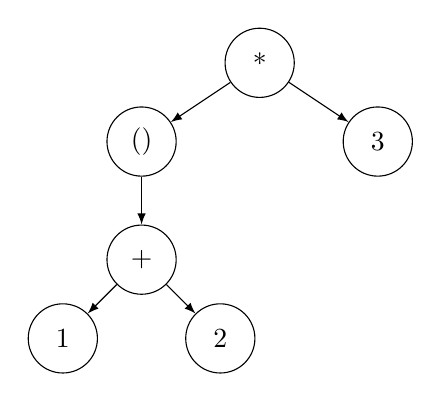
\begin{tikzpicture}
					\node [state] (*) at (8.5,9.5) {*};
					\node [state] (parenthesis) at (7,8.5) {()};
					\node [state] (3) at (10,8.5) {3};
					\node [state] (+) at (7,7) {+};
					\node [state] (1) at (6,6) {1};
					\node [state] (2) at (8,6) {2};
					\path [line] (*) to[left] node[auto] {} (parenthesis);
					\path [line] (*) to[left] node[auto] {} (3);
					\path [line] (parenthesis) to[left] node[auto] {} (+);
					\path [line] (+) to[left] node[auto] {} (1);
					\path [line] (+) to[left] node[auto] {} (2);
				\end{tikzpicture}
			\end{column}
		\end{columns}
	\end{frame}
	
	\begin{frame}
		\frametitle{Dygresja: składnia abstrakcyjna vs składnia konkretna}
		\begin{columns}
			\begin{column}{0.5\textwidth}
				\center{\textbf{Składnia abstrakcyjna}}\newline\newline
			\end{column}
			\begin{column}{0.5\textwidth}
				\center{\textbf{Składnia konkretna}}\newline\newline
			\end{column}
		\end{columns}
		\begin{columns}
			\begin{column}{0.5\textwidth}
				\begin{itemize}
					\item Prostsza
					\item Każde drzewo wyprowadzenia wyznacza jednoznacznie program
					\item Potencjalnie wiele drzew wyprowadzeń dla danego programu
				\end{itemize}
			\end{column}
			\begin{column}{0.5\textwidth}
				\begin{itemize}
					\item Definiowanie wymaga więcej wysiłku
					\item Drzewo wyprowadzenia może zawierać nadmiarowe węzły
					\item Zwykle spełnia dodatkowe własności, umożliwiającą wydajną analizę składniową
					(np. jednoznaczność, LL, LR)
				\end{itemize}

			\end{column}
		\end{columns}
	\end{frame}

	
	\begin{frame}
		\frametitle{Biblioteka}
		\begin{itemize}
		 \item \texttt{obecny()} -- zwraca obecny znak
		 \item \texttt{nastepny()} -- wczytuje kolejny znak z wejścia
		 \item \texttt{wypisz()}, \texttt{wypisz\_liczbe()} -- emituje ciąg znaków/liczbę
		 \item \texttt{error()} -- sygnalizuje błąd i kończy program
		\end{itemize}
	\end{frame}
	
	\begin{frame}[fragile]
		\frametitle{Lekser (analiza leksykalna)}
		\lstset{language=[my]C}
		\begin{lstlisting}
int liczba() {
	int wynik = 0;
	if (!isdigit(obecny())) error();
	while (isdigit(obecny())) {
		wynik = wynik*10 + (obecny() - '0');
		nastepny();
	}
	return wynik;
}`\pause`
bool probuj_znak(char c) {
	if (obecny() != c) return false;
	nastepny();
	return true;
}`\pause`
void znak(char c) {
	if (!probuj_znak(c)) error();
}
		\end{lstlisting}
	\end{frame}
	
	\begin{frame}[fragile]
		\frametitle{Parser (analiza składniowa) + generator kodu}
		\texttt{wyrażenie $\rightarrow$ skladnik | skladnik + wyrazenie}\newline
		\lstset{language=[my]C}
		\lstset{frame=tb}
		\begin{lstlisting}
void wyrazenie() {
	skladnik();
	if (probuj_znak('+')) {
		wyrazenie();
		wypisz("+ ");
	}
}
		\end{lstlisting}
	\end{frame}

	\begin{frame}[fragile]
		\frametitle{Parser (analiza składniowa) + generator kodu}
		\texttt{składnik $\rightarrow$ czynnik | czynnik * skladnik} \newline
		\lstset{language=[my]C}
		\lstset{frame=tb}
		\begin{lstlisting}
void skladnik() {
	czynnik();
	if (probuj_znak('*')) {
		skladnik();
		wypisz("* ");
	}
}
		\end{lstlisting}
	\end{frame}

	\begin{frame}[fragile]
		\frametitle{Parser (analiza składniowa) + generator kodu}
		\texttt{czynnik $\rightarrow$ (wyrażenie) | liczba}
		\lstset{language=[my]C}
		\lstset{frame=tb}
		\begin{lstlisting}
void czynnik() {
	if (probuj_znak('(')) {
		wyrazenie();
		znak(')');
	} else {
		int n = liczba();
		wypisz_liczbe(n);
	}
}
		\end{lstlisting}
	\end{frame}
	
	\begin{frame}
		\frametitle{Brakujące AST}
		Ok, tylko gdzie tu jest drzewo AST?\newline
		\pause
		Jest konstruowane na bieżąco!\newline\newline
		\texttt{1 + 2 * 3}\newline\newline
		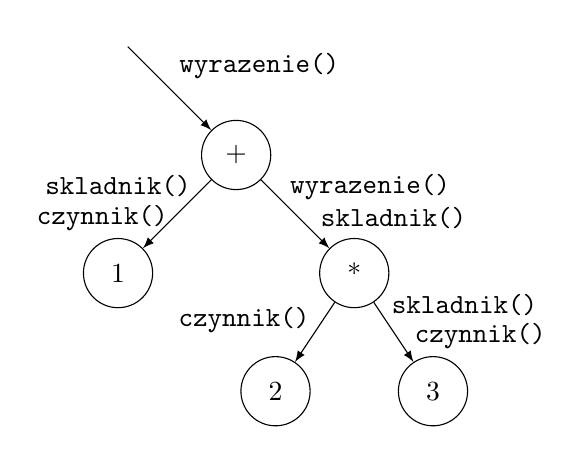
\begin{tikzpicture}
			[scale=1,auto=left]
			\node (start) at (7, 11) {};
			\node [state] (+) at (8.5,9.5) {+};
			\node [state] (1) at (7,8) {1};
			\node [state] (*) at (10,8) {*};
			\node [state] (2) at (9,6.5) {2};
			\node [state] (3) at (11,6.5) {3};
			\path [line] (start) to[left] node[auto] {\texttt{wyrazenie()}} (+);
			\path [line] (+) to[left] node[auto] {} (1);
			\path [line] (+) to[left] node[auto] {} (*);
			\path [line] (*) to[left] node[auto] {} (2);
			\path [line] (*) to[left] node[auto] {} (3);
			\node (label1) at (7, 9.1) {\texttt{skladnik()}};
			\node (label1') at (6.8, 8.7) {\texttt{czynnik()}};
			\node (label*) at (10.2, 9.1) {\texttt{wyrazenie()}};
			\node (label*') at (10.5, 8.7) {\texttt{skladnik()}};
			\node (label2) at (8.6, 7.4) {\texttt{czynnik()}};
			\node (label3) at (11.4, 7.6) {\texttt{skladnik()}};
			\node (label3') at (11.6, 7.2) {\texttt{czynnik()}};
		\end{tikzpicture}
	\end{frame}

	\begin{frame}
	\centering
	\textbf{Demo -- kompilator do ONP}
	\end{frame}
	
	\begin{frame}
		\frametitle{Bardziej skompilowane gramatyki}
		\begin{itemize}
			\item Powyższa gramatyka była bardzo prosta -- nigdy nie potrzebowaliśmy więcej niż następnego znaku
			\item Prawdziwe gramatyki są bardziej skomplikowane
			\item Ogólne metody analizy języków bezkontekstowych -- $O(n^3)$
			\item Języki $LL(k)$ -- mogą być sparsowane zstępująco używając co najwyżej najbliższych $k$ znaków
			\item Języki $LR(k)$ -- mogą być sparsowane wstępująco używając co najwyżej najbliższych $k$ znaków
		\end{itemize}
	\end{frame}
	
	\begin{frame}
		\frametitle{Automatyczne generowanie parserów}
		\begin{itemize}
			\item lex -- generator lekserów
			\item yacc (yet another compiler compiler) -- generator parserów
			\item bison -- nowsza wersja programu yacc
		\end{itemize}
	\end{frame}
	
	\begin{frame}[fragile]
		\frametitle{Notacja infksowa $\rightarrow$ Notacja postfiksowa raz jeszcze}
		\center{lex}
		\begin{lstlisting}[language=c]
[0-9]+  {yylval=atoi(yytext); return LICZBA;}
\n      return 0;
.       return *yytext;
		\end{lstlisting}
		\center{yacc}
		\begin{lstlisting}[language=c]
%token LICZBA
%left '+' '*'
E:  	E '+' E {printf("+ ");}
	|	E '*' E {printf("* ");}
	|	'(' E ')'
	|	LICZBA	{printf("%d ", yylval);}
		\end{lstlisting}

	\end{frame}
	
	\begin{frame}
		\frametitle{Analiza semantyczna}
		\begin{itemize}
			\item Bardzo zależna od języka
			\item Wykrywanie konstrukcji poprawnych składniowo, ale nie mających sensu w semantyce języka
			\item Obliczanie różnych cech poszczególnych węzłów i zapisywanie ich w drzewie
			\item Sprawdzanie typów
			\item Modyfikacja drzewa AST dla operacji implicite (np. rzutowanie w językach słabo typowanych)
		\end{itemize}
	\end{frame}
	
	\begin{frame}
		\frametitle{Generowanie kodu pośredniego}
		\begin{itemize}
			\item Kod dla pewnej abstrakcyjnej maszyny, bliższej maszynie docelowej, ale ukrywającej jej szczegóły
			\item Ułatwia zmianę języka docelowego (np. na inną architekturę procesora)
			\item Wnioskowanie i optymalizacje często są łatwiejsze niż na drzewie AST
			\item Umożliwia wydajniejszą interpretację (uproszczone parsowanie i kompilacja)
		\end{itemize}
	\end{frame}
	
	\begin{frame}
		\frametitle{Rodzaje kodu pośredniego}
		\begin{itemize}
			\item Kod dla maszyny rejestrowej
				\begin{itemize}
					\item LLVM
					\item nlasm
				\end{itemize}
			\item Kod dla maszyny stosowej
				\begin{itemize}
					\item bajtkod .NET -- CIL
					\item bajtkod JVM
					\item bajtkod CPythona
					\item bajtkod WebAssembly
				\end{itemize}
		\end{itemize}
	\end{frame}
	
	\begin{frame}
		\frametitle{LLVM}
		\begin{itemize}
			\item Silnie typowany kod dla maszyny rejestrowej z funkcjami
			\item Standardowy backend dla różnych języków (C, C++, Haskell, Fortran)
			\item Kod trójadresowy: większość instrukcji jest postaci\newline\texttt{wynik = operator typ arg1 arg2}
			\item SSA -- static single assignment, na dowolny rejestr można przypisać wartość tylko raz
		\end{itemize}
	\end{frame}

	\begin{frame}[fragile]
		\frametitle{LLVM -- przykład (ze smurfa [4])}
		\begin{lstlisting}[language=llvm]
define i32 @fact(i32 %n) {
	%c0 = icmp eq i32 %n, 0
	br i1 %c0, label %L0, label %L1
L0:
	ret i32 1
L1:
	%i1 = sub i32 %n, 1
	%i2 = call i32 @fact(i32 %i1)
	%i3 = mul i32 %n, %i2
	ret i32 %i3 
}
		\end{lstlisting}
	\end{frame}
	
	\begin{frame}
		\frametitle{Podstawowe optymalizacje LLVM [5]}
		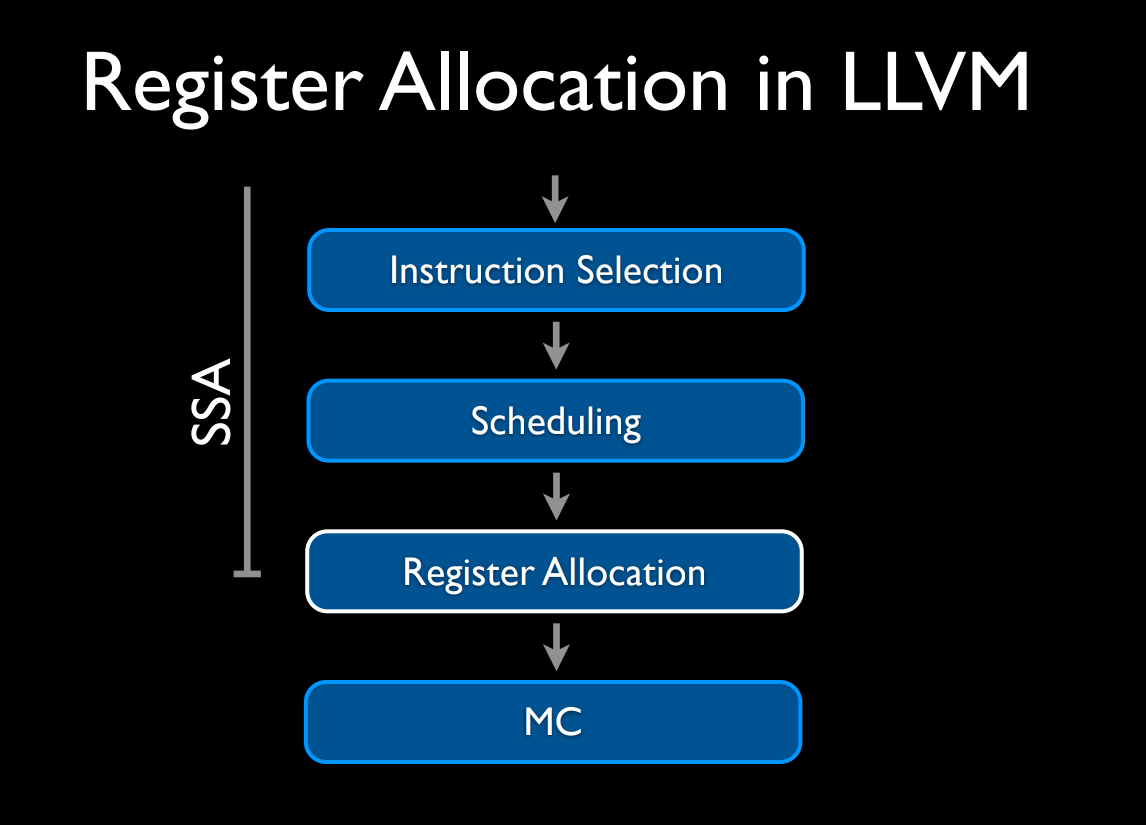
\includegraphics[width=\textwidth]{llvm.png}
	\end{frame}


	\begin{frame}
	 \frametitle{Dziękuję za uwagę}
	 Bibliografia
	 \begin{enumerate}
		\item A.V. Aho, R. Sethi, J.D. Ullman, Kompilatory. Reguły, metody i narzędzia
		\item \url{http://wazniak.mimuw.edu.pl/index.php?title=SW_wyk\%C5\%82ad_2_-_Slajd2}
		\item \url{http://wazniak.mimuw.edu.pl/index.php?title=SW_wyk\%C5\%82ad_2_-_Slajd3}
		\item \url{http://smurf.mimuw.edu.pl/node/797}
		\item \url{https://llvm.org/devmtg/2011-11/Olesen_RegisterAllocation.pdf}
		\item \url{https://llvm.org/devmtg/2016-09/slides/Absar-SchedulingInOrder.pdf}
	 \end{enumerate}
	\end{frame}
\end{document}
